\section{Problem Setting and Repair Method}
\label{sec:framework}
\label{sec:framework:problem}

We study source-grounded repair of a small document-level knowledge graph.
The input consists of a multiset of triples $G$, its source text $X$, a declared
document node $h_0$, and a permitted relation vocabulary $\mathcal R_X$.
The graph is field-oriented: each permitted relation can have at most one
nonempty value for the document. This setting covers tasks such as document metadata and receipt-field extraction.
The reference graph $G^*$ is used only for scoring.

We use literal source matching: a value is supported when it appears in $X$.
Relation correctness and acceptable paraphrases are assessed during evaluation.

Figure~\ref{fig:framework_overview} shows the repository's profile-based
architecture, which connects assessment, routing, and candidate editing.
We first describe the one-call repair pipeline used in the main comparisons.
Section~\ref{sec:impl:optimizer_audit} describes the sequential variant and its
evaluation on fixed proposals.

\begin{figure}[t]
    \centering
    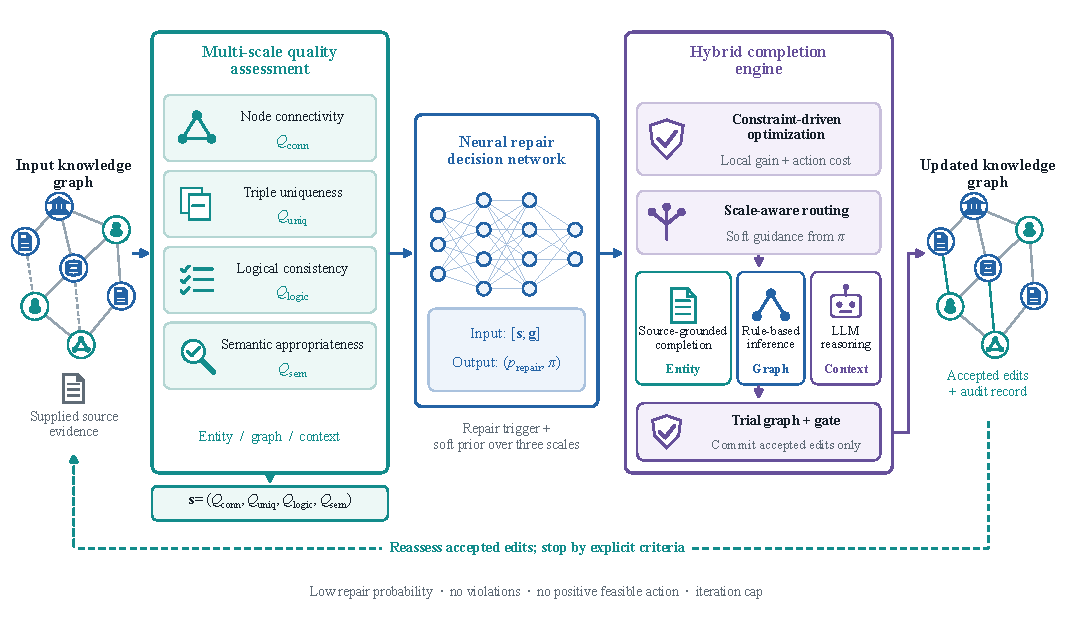
\includegraphics[width=0.98\textwidth]{figure/method/image1.pdf}
    \caption{Profile-based repair architecture. Assessment produces a quality
    profile; the routing policy supplies a repair trigger and a scope prior.
    Model edit bundles and rule proposals pass through trial-state checks;
    each round commits one feasible edit with the highest positive utility.
    The sequential comparison is described in
    Section~\ref{sec:impl:optimizer_audit}.}
    \label{fig:framework_overview}
\end{figure}

\subsection{Structural Normalization and Diagnostic Context}
\label{sec:framework:profile}

Figure~\ref{fig:scale_relationship} groups diagnostic information into local,
graph, and source scopes. For document-field repair, we implement these checks
through duplicate counts, the declared head and relation schema, and source
matching.

\begin{figure}[t]
    \centering
    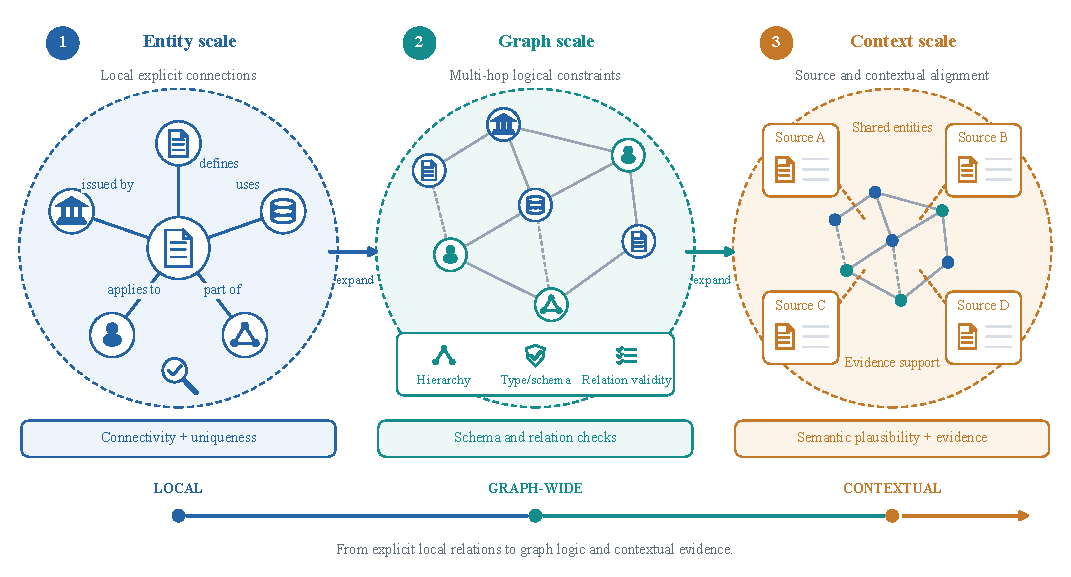
\includegraphics[width=0.98\textwidth]{figure/method/image2.pdf}
    \caption{Three diagnostic scopes. Local checks concern incidence and
    duplicate facts, graph checks concern schema and relation constraints,
    and source checks match values to the associated document. The scopes
    contribute to a shared report. Hierarchy checks use explicit rules.
    The nodes and relations are schematic; the document-field
    checks are specified in Eq.~(\ref{eq:diagnostic_predicates}).}
    \label{fig:scale_relationship}
\end{figure}

A deterministic preprocessor $P$ removes exact duplicates, corrects an edge
when its object equals $h_0$ but its subject does not, and removes triples whose
head or relation violates the supplied schema. Let $G_s=P(G;h_0,\mathcal R_X)$.

For a triple $t=(h,r,o)$, define the executable predicates
\begin{equation}
    \label{eq:diagnostic_predicates}
    H(t)=\mathbf1[h=h_0],\quad
    R(t)=\mathbf1[r\in\mathcal R_X],\quad
    S(t;X)=\mathbf1[o\ne\emptyset\ \wedge\ o\text{ occurs in }X].
\end{equation}
The diagnostic context records duplicate multiplicities, the indices failing
$H$, $R$, or $S$, and the relations observed in $G_s$:
\begin{equation}
    \label{eq:diagnostic_context}
    D(G_s,X)=\big(n_{\mathrm{dup}},I_H,I_R,I_S,\mathcal R(G_s)\big).
\end{equation}
For example, $I_S=\{i:S(t_i;X)=0\}$. The report is computed from the normalized input. Some entries are empty
because preprocessing has already removed the corresponding defect.
The matched experiment tests the effect of adding this report to the prompt.

Allowed fields are optional. A graph can pass all visible checks while
omitting a fact from the source, so the main pipeline makes one model call
for every document.

\subsection{Source-Grounded Candidate Generation}
\label{sec:framework:architecture}

A language model generates an ordered list of proposed triples
\begin{equation}
    \label{eq:proposal_generation}
    C=L_\theta(X,h_0,\mathcal R_X,G_s,D(G_s,X)).
\end{equation}
The model is instructed to return a complete graph, copy source spans, retain
correct fields, and recover missing or corrupted values. A fixed JSON parser
turns malformed responses into empty outputs; failures remain in the
end-to-end denominator. The base setting omits the diagnostic report. Instructions, source, structural input,
model, temperature, and output-token cap remain identical.

\subsection{Constraint-Guided Candidate Selection}
\label{sec:framework:constraints}

From the generated candidates, the gate admits only triples satisfying
Eq.~(\ref{eq:diagnostic_predicates}) and retains at most one triple per relation.
Writing $\operatorname{uniq}(C)$ for exact deduplication in generation order,
let
\begin{equation}
    \label{eq:eligible_candidates}
    C_X=\{t\in\operatorname{uniq}(C):H(t)R(t)S(t;X)=1\}.
\end{equation}
The admissible output family is
\begin{equation}
    \label{eq:admissible_subsets}
    \mathcal F(C_X)=\left\{A\subseteq C_X:
    \sum_{t\in A}\mathbf1[r_t=r]\leq1,\ \forall r\in\mathcal R_X\right\}.
\end{equation}
The gate scans candidates in order and retains the first eligible candidate
for each relation. The resulting $\widehat G$ satisfies
\begin{equation}
    \label{eq:selection_size}
    |\widehat G|=\max_{A\in\mathcal F(C_X)}|A|
    =|\{r:\exists t\in C_X,\ r_t=r\}|.
\end{equation}
Each relation contributes one independent group with capacity one, which
gives Eq.~(\ref{eq:selection_size}). The filter therefore retains the largest
feasible number of supplied candidates. When several values qualify, it uses
generation order to break the tie. We measure factual accuracy and preservation
of input facts separately.

\subsection{Field Definitions and Evidence Lines}
\label{sec:framework:field_evidence}

An allowed relation name may leave its intended value unclear. For example,
a receipt can contain a trading brand, a registered company, a subtotal, and
a final payable amount. In the receipt follow-up, each field has a short
definition shared by all repair methods. All methods also receive the same
numbered source lines.

The evidence-index variant adds line anchors for each field. Fixed patterns
locate company-name terms, address terms and postcodes, date expressions,
and total-amount labels. The index includes each anchor, one preceding line,
and two following lines. It gives the model source locations to reconsider
alongside the current value. The simple baseline receives the same source
and definitions, with the index omitted.

We also make whitespace handling consistent with candidate parsing. Let
$N(s)$ replace each run of whitespace by one space and trim the ends. The
follow-up filter uses
\begin{equation}
    S_{\mathrm{ws}}(t;X)=\mathbf1[|N(o)|>0\ \wedge\
    N(o)\text{ occurs in }N(X)].
\end{equation}
Word boundaries, case, and punctuation are preserved. This predicate replaces
$S$ in the follow-up comparisons; the earlier experiments retain their
original literal check.
